\documentclass[11pt,a4paper]{article}
\usepackage[T1]{fontenc}
\usepackage{lmodern}
\usepackage{amsmath,amssymb,amsthm,mathtools}
\usepackage[margin=1in]{geometry}
\usepackage{graphicx}
\usepackage{float}
\usepackage{booktabs}
\usepackage{xcolor}
\usepackage{enumitem}
\usepackage[colorlinks=true,linkcolor=blue!50!black,citecolor=blue!50!black,urlcolor=blue!50!black]{hyperref}

\theoremstyle{plain}
\newtheorem{theorem}{Theorem}[section]
\newtheorem{proposition}[theorem]{Proposition}
\newtheorem{lemma}[theorem]{Lemma}
\newtheorem{corollary}[theorem]{Corollary}
\theoremstyle{definition}
\newtheorem{definition}[theorem]{Definition}
\newtheorem{postulate}[theorem]{Postulate}
\theoremstyle{remark}
\newtheorem{remark}[theorem]{Remark}

\newcommand{\R}{\mathbb{R}}
\newcommand{\C}{\mathbb{C}}
\newcommand{\N}{\mathbb{N}}
\newcommand{\Z}{\mathbb{Z}}
\newcommand{\cH}{\mathcal{H}}
\newcommand{\dd}{\mathrm{d}}
\newcommand{\Rp}{\R_{>0}}
\newcommand{\lab}[1]{\textsf{\small[#1]}}
\newcommand{\PROVED}{\lab{PROVED}}
\newcommand{\CHECKED}{\lab{CHECKED}}
\newcommand{\NUMERICAL}{\lab{NUMERICAL}}
\newcommand{\CONJ}{\lab{CONJECTURE}}
\newcommand{\HEUR}{\lab{HEURISTIC}}
\newcommand{\OPEN}{\lab{OPEN}}
\renewcommand{\Re}{\operatorname{Re}}
\renewcommand{\Im}{\operatorname{Im}}

\title{The Integers as a Physical System in One Dimension:\\[4pt]
Shadow Pairing, Unitarity, and the Critical Line}
\author{Daniel Toupin\\[2pt]\textit{Golden Physics Project}}
\date{November 2026 --- Round 26 working paper (GPPDiscovery5)}

\begin{document}
\maketitle

\begin{abstract}
\noindent
We take seriously the idea that the positive integers are a physical
system: each integer is a state, each is counted exactly once, and the
complex variable $s$ of the Riemann zeta function is a physical label, the
conformal weight $\Delta$ of a one-dimensional state. Starting from the
shadow pairing $\Delta_5+\Delta_6=2$ of a unitarity cut on the
two-dimensional celestial sphere, we reduce to one dimension, where the
shadow pairing becomes $\Delta+\tilde\Delta=1$, i.e.\ the functional
equation symmetry $s\leftrightarrow 1-s$, and the unitary principal series
of the dilation group and of $SL(2,\R)$ sits on $\Re\Delta=\tfrac12$, the
critical line. We prove a \emph{conditional} theorem: if the nontrivial
zeros of $\xi$ label normalizable states of a self-adjoint generator on a
Hilbert space carrying the reflection $x\mapsto 1/x$ as a symmetry
(the \emph{Physical Integer Postulate}), then every nontrivial zero has real
part $\tfrac12$. We list what the integers supply for free (Tate's theta
as a reflection-invariant vacuum, the functional equation, the absence of
real zeros in $(0,1)$ from ``no negatives'', local positivity at each
prime, reality of $\xi$ on the line, and the fact that Poisson summation
pins the unitary line at exactly $\tfrac12$), and we isolate the single
missing step: constructing that Hilbert space from the integers. That step is
the Hilbert--P\'olya problem, and it is \textbf{open}. Three control
functions satisfy every free property yet have zeros off the line, so any
construction must use the arithmetic fact that every coefficient is exactly
$1$. \textbf{The Riemann Hypothesis is not proved here.}
\end{abstract}

\paragraph{Labels.} Every claim carries one label:
\PROVED{} (complete proof here or in a cited standard source),
\CHECKED{} (classical, verified numerically in \texttt{r26\_checks.py}),
\NUMERICAL{} (computer evidence, not a proof),
\CONJ{}, \HEUR{} (physical reading, not a theorem), \OPEN.
Zeta zeros are never used as inputs to any proof; where they appear it is only
as plot marks.



%=====================================================================
\section{Physical setup and postulates}
\label{sec:setup}

\subsection{The picture}

A physicist meets $\zeta(s)=\sum_{n\ge1}n^{-s}$ and sees a partition
function. Give the state $|n\rangle$ the energy $\log n$. Then
\begin{equation}\label{eq:primon}
\zeta(s)=\sum_{n\ge1}e^{-s\log n}=\operatorname{Tr}e^{-sH},
\qquad H|n\rangle=(\log n)|n\rangle ,
\end{equation}
for $\Re s>1$. This is Julia's ``free Riemann gas'' (the primon gas)
\cite{Julia1990,Spector1990}: the primes are bosonic modes of energy
$\log p$, a state of the gas is a choice of occupation numbers, and unique
factorization says that every integer appears in the spectrum
\emph{exactly once}. The Euler product
\begin{equation}\label{eq:euler}
\zeta(s)=\prod_p\bigl(1-p^{-s}\bigr)^{-1}
\end{equation}
is the statement that the gas is free: the partition function factorizes
over independent prime oscillators \PROVED{} (Euler; unique factorization).

Write $s=\sigma+it$. Then each term is
\begin{equation}\label{eq:arrow}
n^{-s}=n^{-\sigma}\,e^{-it\log n}:
\end{equation}
an arrow of positive length $n^{-\sigma}$ rotating at angular frequency
$\log n$. The real part $\sigma$ is an inverse temperature, and the imaginary
part $t$ is a real time. For $\sigma>1$,
\[
\frac{\zeta(\sigma+it)}{\zeta(\sigma)}=\bigl\langle e^{-itH}\bigr\rangle_{\sigma}
\]
is the return (Loschmidt) amplitude of the Gibbs state at inverse
temperature $\sigma$ \PROVED{} (definition). A zero of $\zeta$ is a time at
which the thermal ensemble of arrows interferes to exactly nothing. In the
language of statistical mechanics, the zeros are the Fisher zeros of the gas
at complex temperature. Their location is the subject of Lee--Yang type
theorems \cite{LeeYang1952}, and of their modern dynamical cousins
\cite{Heyl2013}. Julia already drew this analogy \cite{Julia1990}. See also
Bost--Connes \cite{BostConnes1995} and Knauf \cite{Knauf1999}.

\subsection{Daniel's postulates}

We state the physical input as four postulates. They are physical
\emph{assumptions}, not theorems, and Section~\ref{sec:main} shows exactly
which mathematical statement they need to become.

\begin{enumerate}[label=\textbf{(P\arabic*)},leftmargin=3em]
\item \textbf{The integers are physical.} The natural numbers are not a
human bookkeeping device. They are the spectrum of a physical system, as
in~\eqref{eq:primon}.
\item \textbf{Each is counted once.} Every state $|n\rangle$ has weight
exactly $1$. In arithmetic this is the Euler product~\eqref{eq:euler} with
every Dirichlet coefficient equal to $1$.
\item \textbf{Addition and multiplication are two measurements of one state.}
The additive structure of $\Z$ (translations and Fourier analysis) and the
multiplicative structure (dilations and the Mellin transform) act on one
and the same object. Section~\ref{sec:free} shows that object to be Tate's
theta function, with the Gaussian as its vacuum.
\item \textbf{There are no negatives.} Starting from positive numbers and
multiplying, one never produces a negative number. Every cancellation in
$\sum n^{-s}$ is therefore a \emph{rotation} of positive arrows, never a
subtraction. (Even the sign $(-1)^{n-1}$ in the alternating series
$\eta(s)$ is a half-turn, $e^{i\pi(n-1)}$.)
\end{enumerate}
\noindent
And the organizing principle:
\begin{enumerate}[label=\textbf{(S)},leftmargin=3em]
\item \textbf{$s$ is physical.} The variable $s$ is the conformal weight
$\Delta$ of a physical (normalizable) one-dimensional state.
\end{enumerate}

The program of this paper is to show that (S), made precise, \emph{forces}
the critical line (Theorem~\ref{thm:main}). It is also to show that
(P1)--(P4), as far as anyone can currently prove, supply everything
\emph{except} (S) itself (Sections~\ref{sec:free}--\ref{sec:gap}).

%=====================================================================
\section{From the celestial sphere to the line: the shadow pairing}
\label{sec:reduction}

\subsection{The two-dimensional starting point}

In Daniel's August 2026 paper on loop amplitudes from unitarity cuts in
celestial Mellin space \cite{ToupinLoops2026}, the two-particle massless cut
is written on the celestial sphere $S^2$. Its Mellin image is
\begin{equation}\label{eq:phi2d}
\Phi(\Delta_5,\Delta_6;M)=\frac1{8\pi}\Bigl(\frac M2\Bigr)^{\Delta_5+\Delta_6-2}
\frac{\Gamma(\Delta_5)\Gamma(\Delta_6)}{\Gamma(\Delta_5+\Delta_6)} .
\end{equation}
The cut is exactly scale invariant on the locus
\[
\Delta_5+\Delta_6=2 ,
\]
which is the \emph{shadow pairing} $\Delta\leftrightarrow 2-\Delta$ of a
two-dimensional conformal field theory. On the principal series
$\Delta_5=1+i\lambda$, the cut pair is a shadow pair, and the phase-space
factor is
\begin{equation}\label{eq:P2d}
\Gamma(1+i\lambda)\Gamma(1-i\lambda)=\frac{\pi\lambda}{\sinh\pi\lambda}
=\bigl|\Gamma(1+i\lambda)\bigr|^2>0
\end{equation}
\CHECKED{} (reflection formula; \cite{ToupinLoops2026}, Eq.~(plambda)). The
principal series $\Delta=1+i\lambda$ is the set of weights of
delta-normalizable massless conformal primary wavefunctions
\cite{PasterskiShaoStrominger2017}. It is the unitary principal series of the
Lorentz group $SL(2,\C)$ acting on $S^2$ \cite{Dobrev1977}.

The structural reason~\eqref{eq:P2d} is positive is worth stating plainly.
On the unitary line the shadow partner of $\Delta$ is its complex conjugate,
$2-\Delta=\bar\Delta$, so the product of the two legs is a modulus squared.
\emph{Shadow pairing plus unitarity equals complex conjugation.}

\subsection{Dimensional reduction to $d=1$}

For a conformal theory in $d$ dimensions the shadow of $\Delta$ is
$d-\Delta$, and the unitary principal series is $\Delta=\tfrac d2+i\lambda$
\cite{Dobrev1977}. Going from the sphere ($d=2$) to the line ($d=1$):
\begin{center}
\begin{tabular}{lcc}
\toprule
 & $d=2$ (celestial sphere) & $d=1$ (line / half-line)\\
\midrule
shadow pairing & $\Delta+\tilde\Delta=2$ & $\Delta+\tilde\Delta=1$\\
unitary principal series & $\Delta=1+i\lambda$ & $\Delta=\tfrac12+i\lambda$\\
conjugation on the unitary line & $\tilde\Delta=\bar\Delta$ & $\tilde\Delta=\bar\Delta$\\
cut factor $\Gamma(\Delta)\Gamma(\tilde\Delta)/\Gamma(d)$ &
$\dfrac{\pi\lambda}{\sinh\pi\lambda}$ & $\dfrac{\pi}{\cosh\pi\lambda}$\\
symmetry group & $SL(2,\C)$ & $SL(2,\R)\supset$ dilations\\
\bottomrule
\end{tabular}
\end{center}
In $d=1$, the shadow pairing $\Delta\leftrightarrow1-\Delta$ is
\emph{literally} the symmetry $s\leftrightarrow1-s$ of Riemann's functional
equation, and the unitary line $\Re\Delta=\tfrac12$ is \emph{literally} the
critical line. This is the observation that drives the paper \HEUR{} (as a
physical identification; the group theory is standard).

The one-dimensional cut factor is the Euler Beta function at shadow-paired
arguments,
\begin{equation}\label{eq:B1d}
B(\Delta,1-\Delta)=\Gamma(\Delta)\Gamma(1-\Delta)=\frac{\pi}{\sin\pi\Delta}.
\end{equation}
\begin{proposition}[the 1D cut factor detects the unitary dual]\label{prop:cut1d}
For $\Delta=\beta+i\gamma$ with $0<\beta<1$, the factor
$\Gamma(\Delta)\Gamma(1-\Delta)$ is real if and only if $\beta=\tfrac12$ or
$\gamma=0$. On $\beta=\tfrac12$ it equals $\pi/\cosh(\pi\gamma)>0$. On
$\gamma=0$ it equals $\pi/\sin(\pi\beta)>0$. \PROVED
\end{proposition}
\begin{proof}
$\sin(\pi\beta+i\pi\gamma)=\sin\pi\beta\cosh\pi\gamma+i\cos\pi\beta\sinh\pi\gamma$.
For $0<\beta<1$ this is real iff $\cos\pi\beta\sinh\pi\gamma=0$, i.e.\
$\beta=\tfrac12$ or $\gamma=0$, and in both cases it is positive. Then use
\eqref{eq:B1d}.
\end{proof}
\noindent
The two loci of Proposition~\ref{prop:cut1d}, the line $\Re\Delta=\tfrac12$
and the real segment $(0,1)$, are exactly the principal and complementary
series of $SL(2,\R)$ (Section~\ref{sec:dual}). So the 1D phase-space factor
is positive precisely on the unitary dual and is complex everywhere else in
the strip. That fact will reappear as Lemma~\ref{lem:casimir}. The positivity
of the cut is the positivity of the norm.

%=====================================================================
\section{The one-dimensional Hilbert space and its unitary dual}
\label{sec:dual}

\subsection{States on the half-line}

The 1D arena is the half-line $\Rp$, the space of scales. Take
\begin{equation}\label{eq:H}
\cH_0=L^2(\Rp,\dd x),\qquad (U(a)f)(x)=a^{-1/2}f(x/a),\quad a>0 .
\end{equation}
$U$ is a strongly continuous unitary representation of the dilation group
$\Rp^\times$. Its self-adjoint generator is the 1D \emph{dilatation
operator} (the quantized $xp$ of Berry--Keating \cite{BerryKeating1999} and
Connes \cite{Connes1999}),
\begin{equation}\label{eq:D}
D=i\Bigl(x\frac{\dd}{\dd x}+\frac12\Bigr),\qquad U(e^{\tau})=e^{-i\tau D}.
\end{equation}
The scaling ``plane waves'' $e_\Delta(x)=x^{-\Delta}$ satisfy
\begin{equation}\label{eq:eig}
D\,e_\Delta=-i\bigl(\Delta-\tfrac12\bigr)e_\Delta ,
\qquad\text{so}\qquad \Delta=\tfrac12+iE\iff \text{eigenvalue }E .
\end{equation}

\paragraph{The reflection.} Define the antilinear map
\begin{equation}\label{eq:Theta}
(\Theta f)(x)=x^{-1}\,\overline{f(1/x)} .
\end{equation}

\begin{lemma}[reflection]\label{lem:theta}
\PROVED{} On $\cH_0$:
\begin{enumerate}[label=(\roman*)]
\item $\Theta$ is an antiunitary involution: $\|\Theta f\|=\|f\|$ and $\Theta^2=1$.
\item $\Theta U(a)\Theta=U(a)^{-1}$, equivalently $\Theta D\Theta=D$:
the reflection commutes with the generator.
\item $\Theta e_\Delta=e_{1-\bar\Delta}$: the reflection sends a weight to its
conjugated shadow, and fixes exactly the weights with $\Re\Delta=\tfrac12$.
\item On Mellin transforms $\tilde f(s)=\int_0^\infty f(x)x^{s-1}\dd x$:
$\widetilde{\Theta f}(s)=\overline{\tilde f(1-\bar s)}$.
\end{enumerate}
\end{lemma}
\begin{proof}
(i) With $y=1/x$,
$\int_0^\infty x^{-2}|f(1/x)|^2\dd x=\int_0^\infty|f(y)|^2\dd y$. Also
$\Theta^2f(x)=x^{-1}\overline{(\Theta f)(1/x)}=x^{-1}\cdot x\,f(x)=f(x)$.
(ii) $\Theta U(a)\Theta f(x)=x^{-1}a^{-1/2}\overline{(\Theta f)(1/(ax))}
=x^{-1}a^{-1/2}(ax)f(ax)=a^{1/2}f(ax)=(U(a^{-1})f)(x)$. Since $\Theta$ is
antilinear, $\Theta e^{-i\tau D}\Theta=e^{+i\tau\,\Theta D\Theta}$, and
comparing with $U(e^{-\tau})=e^{i\tau D}$ gives $\Theta D\Theta=D$.
(iii) $x^{-1}\overline{(1/x)^{-\Delta}}=x^{-1}x^{\bar\Delta}=x^{-(1-\bar\Delta)}$.
And $1-\bar\Delta=\Delta$ iff $\Re\Delta=\tfrac12$.
(iv) Substitute $y=1/x$ in
$\int x^{-1}\overline{f(1/x)}x^{s-1}\dd x=\int\overline{f(y)}\,y^{-s}\dd y
=\overline{\int f(y)y^{-\bar s}\dd y}=\overline{\tilde f(1-\bar s)}$.
\end{proof}

Physically, $\Theta$ is a time reversal for the dilation ``clock''. It is
antiunitary and commutes with the Hamiltonian $D$. Item (iii) is the
operator form of the mirror symmetry $\xi(1-\bar s)=\overline{\xi(s)}$ that
Round 25 drew (Section~\ref{sec:outlook}).

\subsection{What ``physical weight'' means}

Every complex $\Delta$ gives a perfectly good function $x^{-\Delta}$ and
satisfies~\eqref{eq:eig} formally. Being an eigenfunction is not the
physics. \emph{Normalizability} is.

\begin{lemma}[only the unitary line is normalizable]\label{lem:norm}
\PROVED{} Let $\Delta=\beta+i\lambda$, and let $\chi\in C_c^\infty(\R)$ be a
bump with $\chi(0)=1$. Put $\chi_L(x)=\chi(\log x/L)$ and
$\phi_L=\chi_L e_\Delta\in\cH_0$.
\begin{enumerate}[label=(\roman*)]
\item If $\beta=\tfrac12$, then $\|\phi_L\|^2=L\|\chi\|^2_{L^2(\R)}$ grows
linearly, and $\psi_L=\phi_L/\|\phi_L\|$ satisfies
$\|(D-\lambda)\psi_L\|=O(L^{-1})$. So $\lambda\in\sigma(D)$, and
$e_{1/2+i\lambda}$ is delta-normalizable:
$\langle e_{1/2+i\lambda},e_{1/2+i\lambda'}\rangle=2\pi\delta(\lambda-\lambda')$.
\item If $\beta\neq\tfrac12$, then $\|\phi_L\|^2$ grows like
$e^{|1-2\beta|cL}$ for some $c>0$, and no sequence of unit vectors can be an
approximate eigenvector for the value $z=\lambda-i(\beta-\tfrac12)$:
\begin{equation}\label{eq:gap}
\|(D-z)\psi\|\ \ge\ |\beta-\tfrac12|\,\|\psi\|\qquad\text{for all }\psi\in\operatorname{dom}D .
\end{equation}
\end{enumerate}
\end{lemma}
\begin{proof}
Go to $u=\log x$. The map $f\mapsto g$, $g(u)=e^{u/2}f(e^u)$, is unitary
$L^2(\Rp,\dd x)\to L^2(\R,\dd u)$, and it carries $D$ to $i\,\dd/\dd u$ (the
$\tfrac12$ in~\eqref{eq:D} exactly cancels the Jacobian). It carries
$e_\Delta$ to $e^{(\frac12-\beta)u}e^{-i\lambda u}$. (i) For $\beta=\tfrac12$
the image of $\phi_L$ is $\chi(u/L)e^{-i\lambda u}$, with norm$^2$
$L\|\chi\|^2$. Moreover $(i\,\dd/\dd u-\lambda)$ of it is
$iL^{-1}\chi'(u/L)e^{-i\lambda u}$, of norm $L^{-1/2}\|\chi'\|$, so after
normalizing we get $O(L^{-1})$. The delta normalization is Fourier
inversion in $u$. (ii) The norm$^2$ is
$\int\chi(u/L)^2e^{(1-2\beta)u}\dd u$, which grows exponentially in $L$. For
\eqref{eq:gap}, use the standard inequality for self-adjoint $D$:
$\Im\langle(D-z)\psi,\psi\rangle=-\Im z\,\|\psi\|^2$, hence
$\|(D-z)\psi\|\,\|\psi\|\ge|\Im z|\,\|\psi\|^2$, with
$\Im z=-(\beta-\tfrac12)$.
\end{proof}

Inequality~\eqref{eq:gap} is the whole mechanism in one line: \emph{a
self-adjoint Hamiltonian has a spectral gap of size $|\Im z|$ around every
non-real number.} Off-line weights are a finite distance $|\beta-\tfrac12|$
away from anything physical.

\subsection{Why the line is at exactly $\tfrac12$}

Bellissard \cite{Bellissard2017} made a sharp point about any dilation
approach. On the weighted space $L^2(\Rp,x^\alpha\dd x)$ the unitary dilation
is $a^{-(1+\alpha)/2}f(x/a)$, and the physical line moves to
$\Re\Delta=\tfrac{1+\alpha}2$. So the number $\tfrac12$ is not automatic. Here
the integers themselves pick the weight.

\begin{lemma}[Poisson summation pins $\alpha=0$]\label{lem:alpha}
\PROVED{} For each real $\alpha$, the map
$\Theta_\alpha f(x)=x^{-(1+\alpha)}\overline{f(1/x)}$ is an antiunitary
involution of $L^2(\Rp,x^\alpha\dd x)$. It fixes the line
$\Re\Delta=\tfrac{1+\alpha}2$. The Jacobi theta function
$T(x)=\sum_{n\in\Z}e^{-\pi n^2x^2}$ satisfies $\Theta_\alpha T=T$ if and only
if $\alpha=0$.
\end{lemma}
\begin{proof}
Unitarity is the computation of Lemma~\ref{lem:theta}(i), with the weight
carried along. Poisson summation applied to the Gaussian gives
$T(x)=x^{-1}T(1/x)$ (Jacobi; \cite{Titchmarsh1986}, \S2.6). Then
$\Theta_\alpha T(x)=x^{-(1+\alpha)}T(1/x)=x^{-\alpha}T(x)$, which equals
$T(x)$ for all $x$ iff $\alpha=0$.
\end{proof}
\noindent
\emph{Physically:} the additive self-duality of the Gaussian (it is its own
Fourier transform), summed over the integers, fixes the reflection to be
exactly~\eqref{eq:Theta}. That reflection is unitary only on $L^2(\Rp,\dd x)$,
whose unitary line is $\tfrac12$. Addition fixes the stage on which
multiplication is unitary. This is (P3) in action \PROVED{} (as stated) and
\HEUR{} (as interpretation).

\subsection{The unitary dual}

\begin{proposition}[dilation group]\label{prop:dil}
\PROVED{} The irreducible unitary representations of $\Rp^\times$ are the
characters $a\mapsto a^{iE}$, $E\in\R$. In weight language they are
$\Delta=\tfrac12+iE$. A vector $v\neq0$ with $U(a)v=a^{\Delta-1/2}v$ for all
$a$, in any unitary representation, forces $\Re\Delta=\tfrac12$.
\end{proposition}
\begin{proof}
$\Rp^\times\cong(\R,+)$ is abelian, so its irreducible unitary
representations are one-dimensional, and continuous unitary characters of
$\R$ are $\tau\mapsto e^{iE\tau}$ with $E$ real. For the last claim,
$\|v\|=\|U(a)v\|=a^{\Re\Delta-1/2}\|v\|$ for all $a>0$.
\end{proof}

\begin{proposition}[$SL(2,\R)$; Bargmann]\label{prop:sl2}
\PROVED{} \cite{Bargmann1947,Lang1975,Knapp1986}. Label an irreducible
representation of $SL(2,\R)$ by its Casimir eigenvalue $C=\Delta(1-\Delta)$.
The nontrivial irreducible unitary representations are:
the principal series $\Delta=\tfrac12+i\lambda$ ($C=\tfrac14+\lambda^2$);
the complementary series $\Delta\in(0,1)$ real ($0<C<\tfrac14$); and the
discrete series (and limits) with $\Delta$ a positive integer or half-integer
\cite{Knapp1986}. In every case $C$ is \emph{real}.
\end{proposition}

\begin{lemma}[the Casimir of a unitary irrep is real]\label{lem:casimir}
\PROVED{} If $\pi$ is an irreducible unitary representation of $SL(2,\R)$
(or of its universal cover), its Casimir acts on smooth vectors as a real
scalar. For $\Delta=\beta+i\gamma$,
\[
\Im\bigl[\Delta(1-\Delta)\bigr]=\gamma(1-2\beta),
\]
which vanishes iff $\beta=\tfrac12$ or $\gamma=0$.
\end{lemma}
\begin{proof}
By Schur's lemma for irreducible unitary representations (Harish-Chandra's
theorem on admissible representations \cite{Knapp1986}), the Casimir
$\Omega$ acts on smooth vectors as a scalar $c$. In a basis $H,X,Y$ of
$\mathfrak{sl}_2(\R)$, $\Omega$ is a real quadratic expression,
$\Omega=\tfrac14H^2+\tfrac12(XY+YX)$ up to normalization. Each Lie algebra
element acts skew-symmetrically on smooth vectors, because $\pi$ is
unitary. So products of two of them, with real coefficients, are
symmetric, and $\Omega$ is symmetric. Then for smooth $v\ne0$,
$c\|v\|^2=\langle\Omega v,v\rangle=\langle v,\Omega v\rangle=\bar c\|v\|^2$.
The formula for $\Im[\Delta(1-\Delta)]$ is algebra.
\end{proof}
\noindent
Note the exact match with Proposition~\ref{prop:cut1d}: the 1D cut factor
is real on the same two loci on which the Casimir is real.

%=====================================================================
\section{The main conditional theorem}
\label{sec:main}

We now turn (S) into mathematics. Let $\mathcal Z$ denote the multiset of
nontrivial zeros of $\zeta$, i.e.\ the zeros of
\[
\xi(s)=\tfrac12 s(s-1)\pi^{-s/2}\Gamma(s/2)\zeta(s),
\]
which is entire. It is classical that $\mathcal Z$ lies in the open strip
$0<\Re s<1$ \PROVED{} (Hadamard, de la Vall\'ee Poussin; \cite{Titchmarsh1986},
Ch.~III).

\begin{postulate}[Physical Integer Postulate, Hilbert-space form]\label{pip}
There exist a complex Hilbert space $\cH$, a self-adjoint operator $H$ on
$\cH$, and an antiunitary involution $\Theta$ with $\Theta H\Theta=H$, such
that for every $\rho\in\mathcal Z$ there is a \emph{normalizable} state
$0\ne v_\rho\in\operatorname{dom}H$ of conformal weight $\Delta=\rho$:
\begin{equation}\label{eq:pip}
H v_\rho=-i\bigl(\rho-\tfrac12\bigr)v_\rho .
\end{equation}
\end{postulate}
\noindent
The normalization in~\eqref{eq:pip} is the one forced by Lemma~\ref{lem:alpha}:
weight $\Delta$ means eigenvalue $-i(\Delta-\tfrac12)$ of the dilatation
generator, exactly as in~\eqref{eq:eig}.

\begin{postulate}[Physical Integer Postulate, representation form]\label{pipR}
For every $\rho\in\mathcal Z$ there is an irreducible unitary representation
$\pi_\rho$ of $SL(2,\R)$, or of its universal cover, whose Casimir eigenvalue is
$\rho(1-\rho)$.
\end{postulate}

\begin{theorem}[physical weights lie on the critical line]\label{thm:main}
\PROVED{} (as a conditional statement).
\begin{enumerate}[label=(\alph*)]
\item If Postulate~\ref{pip} holds, then $\Re\rho=\tfrac12$ for every
$\rho\in\mathcal Z$.
\item If Postulate~\ref{pipR} holds, then $\Re\rho=\tfrac12$ for every
$\rho\in\mathcal Z$.
\end{enumerate}
In either case, the Riemann Hypothesis follows.
\end{theorem}

\begin{proof}
(a) Let $\rho=\beta+i\gamma\in\mathcal Z$ and $z=-i(\rho-\tfrac12)
=\gamma-i(\beta-\tfrac12)$. Since $H$ is self-adjoint, $\langle Hv,v\rangle$
is real for every $v\in\operatorname{dom}H$. Hence
\[
0=\Im\langle(H-z)v_\rho,v_\rho\rangle=-\Im z\,\|v_\rho\|^2
=(\beta-\tfrac12)\|v_\rho\|^2 .
\]
Since $v_\rho\neq0$, we get $\beta=\tfrac12$. (This is~\eqref{eq:gap} with
$\psi=v_\rho$.) The symmetry $\Theta$ is not needed for the conclusion, but
it is consistent with it. By Lemma~\ref{lem:theta}(iii), $\Theta v_\rho$ has
weight $1-\bar\rho$, which is again a zero, by the functional equation
(Proposition~\ref{prop:fe}). Under the postulate $1-\bar\rho=\rho$, so the
functional-equation quartet $\{\rho,\bar\rho,1-\rho,1-\bar\rho\}$ collapses
to a conjugate pair, and $\Theta$ acts within each energy level, as a time
reversal should.

(b) Let $\rho=\beta+i\gamma\in\mathcal Z$. By Lemma~\ref{lem:casimir},
$\gamma(1-2\beta)=0$. So either $\beta=\tfrac12$, or $\gamma=0$ and $\rho$ is
a real zero in $(0,1)$. The latter is impossible by
Proposition~\ref{prop:noreal} below, which uses only (P4). Hence $\beta=\tfrac12$.

Since $\mathcal Z$ is exactly the set of nontrivial zeros, $\Re\rho=\tfrac12$
for all of them is the Riemann Hypothesis.
\end{proof}

\paragraph{Real zeros in $(0,1)$.} Part (b) deserves a comment. A real
$\Delta\in(0,1)$ is a perfectly good unitary weight: it is the complementary
series, unitary with respect to a non-local intertwining inner product. So
the representation-theoretic postulate alone cannot exclude real zeros. The
integers exclude them directly:

\begin{proposition}[no negatives $\Rightarrow$ no real zeros in $(0,1)$]\label{prop:noreal}
\PROVED{} For $0<\sigma<1$, $\zeta(\sigma)<0$. In particular $\xi$ has no
zeros in $(0,1)$ \cite{Titchmarsh1986,Edwards1974}.
\end{proposition}
\begin{proof}
For $\sigma>0$,
$\eta(\sigma)=\sum_{n\ge1}(-1)^{n-1}n^{-\sigma}=(1-2^{1-\sigma})\zeta(\sigma)$
(analytic continuation from $\sigma>1$). The series is alternating, with
strictly decreasing positive terms. Grouping it in pairs,
$\eta(\sigma)=\sum_{k\ge1}\bigl[(2k-1)^{-\sigma}-(2k)^{-\sigma}\bigr]>0$.
For $\sigma<1$, $1-2^{1-\sigma}<0$, so $\zeta(\sigma)<0$. The factor
$\tfrac12s(s-1)\pi^{-s/2}\Gamma(s/2)$ does not vanish on $(0,1)$.
\end{proof}
\noindent
This is (P4) in its purest form. At $t=0$ nothing rotates. The arrows of
$\eta$ point alternately forward and backward (a half-turn), with strictly
shrinking lengths, so they cannot close up. \emph{With positive lengths and
no rotation, there is no cancellation.} Off the real axis, the arrows
rotate, and positivity of the lengths alone no longer prevents closure.

\begin{remark}[honesty about the strength of Theorem~\ref{thm:main}]\label{rem:tauto}
\PROVED. The converse also holds: if RH is true, take
$\cH=\ell^2(\mathcal Z)$ with $H$ diagonal, $Hv_\rho=\Im(\rho)v_\rho$ (real),
and $\Theta$ complex conjugation of coordinates in the basis $(v_\rho)$, which commutes with the real diagonal $H$.
So Postulate~\ref{pip} is \emph{equivalent} to RH. Theorem~\ref{thm:main} is
logically easy. Its value is that it says precisely \emph{what} a physical
derivation must deliver: a Hilbert space and a self-adjoint generator built
from the integers, with the zeros as normalizable weights, and with no
knowledge of the zeros used in the construction. All the difficulty lives
in that sentence. This is the Hilbert--P\'olya program
(Section~\ref{sec:gap}).
\end{remark}

%=====================================================================
\section{What the integers supply for free}
\label{sec:free}

Everything in this section is proved, and none of it uses zeros.

\subsection{Tate's theta and the Gaussian vacuum}

The Gaussian $g(x)=e^{-\pi x^2}$ is the ground state of the harmonic
oscillator and is its own Fourier transform. Let the integers act on it by
dilation and add the results, each integer once:
\[
\omega(x)=\sum_{n\ge1}g(nx)=\sum_{n\ge1}e^{-\pi n^2x^2},\qquad
T(x)=1+2\omega(x)=\sum_{n\in\Z}e^{-\pi n^2x^2}.
\]
\begin{proposition}[Riemann's second proof, in this language]\label{prop:fe}
\PROVED{} \cite{Riemann1859,Titchmarsh1986,Tate1950}.
\begin{enumerate}[label=(\roman*)]
\item (Additive measurement.) $T=\Theta T$, i.e.\ $T(x)=x^{-1}T(1/x)$
(Poisson summation).
\item (Multiplicative measurement.) For $\Re s>1$,
$\displaystyle\int_0^\infty\omega(x)x^{s-1}\dd x=\tfrac12\pi^{-s/2}\Gamma(s/2)\zeta(s)$,
and the Euler product~\eqref{eq:euler} holds.
\item (Consequence.) $\xi$ extends to an entire function with
$\xi(s)=\xi(1-s)$ and $\overline{\xi(\bar s)}=\xi(s)$.
\end{enumerate}
\end{proposition}
\noindent
\emph{Proof sketch} (standard). Split the Mellin integral at $x=1$, apply (i)
on $(0,1)$, and use $\omega=\tfrac12(T-1)$. The result is
$\tfrac12\pi^{-s/2}\Gamma(s/2)\zeta(s)=-\frac1s-\frac1{1-s}
+\int_1^\infty\omega(x)(x^{s-1}+x^{-s})\dd x$, which is visibly symmetric
under $s\mapsto1-s$ and entire apart from the two poles. Those poles are
cancelled by $\tfrac12s(s-1)$. \qed

The physics reading of (P3) is now exact. \emph{One state, $T$, is
measured two ways.} Under the additive measurement (Fourier, Poisson) it is
reflection invariant, $T=\Theta T$. Under the multiplicative measurement
(Mellin) it \emph{is} the completed zeta function. The functional equation
is the statement that the two measurements are compatible. The constant
term $1$ that separates $T$ from $2\omega$ (the $n=0$ ``vacuum'' mode) is
what produces the two poles of $\pi^{-s/2}\Gamma(s/2)\zeta(s)$. The
reflection~\eqref{eq:Theta} of Section~\ref{sec:dual} is \emph{exactly}
Poisson summation (Lemma~\ref{lem:alpha}).

\subsection{Reality on the line and the mirror}

\begin{corollary}\label{cor:real}
\PROVED{} $\xi(1-\bar s)=\overline{\xi(s)}$ for all $s$, and hence
$\xi(\tfrac12+it)\in\R$ for every real $t$. \CHECKED{} numerically to
$10^{-41}$ relative error in \texttt{r26\_checks.py}.
\end{corollary}
\noindent
This is the operator identity $\Theta e_\Delta=e_{1-\bar\Delta}$
(Lemma~\ref{lem:theta}(iii)) seen through the Mellin transform
(Lemma~\ref{lem:theta}(iv)). It is why ``the imaginary part disappears''
on the whole critical line, and not only at the zeros.

\subsection{Local positivity at every prime}

Each Euler factor is a single bosonic oscillator. On the critical line,
with $r=p^{-1/2}$ and $\vartheta=t\log p$,
\begin{equation}\label{eq:poisson}
K_p(t)=\frac{1-p^{-1}}{|1-p^{-1/2-it}|^2}
=\frac{1-r^2}{1-2r\cos\vartheta+r^2}
=1+2\sum_{k\ge1}p^{-k/2}\cos(kt\log p).
\end{equation}
\begin{proposition}[each prime is locally positive]\label{prop:local}
\PROVED{} $K_p$ is the Poisson kernel of the unit disc at radius
$p^{-1/2}$. Hence $K_p>0$, and $K_p-1$ is a positive-definite function of
$t$ (a cosine series with positive coefficients; Bochner). \CHECKED{} in
\texttt{r26\_checks.py}.
\end{proposition}
\noindent
This is the content of Daniel's Python model (per-prime kernels, each
positive-definite), and it is correct. The difficulty is the sign with
which the primes enter the global positivity criterion. Weil's explicit
formula \cite{Weil1952,Bombieri2000} for an even test function $h$ with
Fourier transform $\hat h$ reads, schematically,
\begin{equation}\label{eq:weil}
\sum_{\rho}\hat h\bigl(\tfrac{\rho-1/2}{i}\bigr)
=\underbrace{\hat h(\tfrac i2)+\hat h(-\tfrac i2)}_{\text{pole}}
\;+\;\underbrace{(\text{archimedean term})}_{\Gamma\text{-factor}}
\;-\;\underbrace{2\sum_{n\ge2}\frac{\Lambda(n)}{\sqrt n}h(\log n)}_{\text{primes}},
\end{equation}
and $\sum_{p,k}\log p\,p^{-k/2}\cos(kt\log p)=\tfrac12\sum_p\log p\,(K_p(t)-1)$
is exactly the prime sum in~\eqref{eq:weil} written at frequency $t$
\PROVED{} (rearrangement of $-\zeta'/\zeta$, valid for $\Re s>1$ and in the
distributional sense on the line). Weil's criterion says RH holds iff the
left side is $\ge0$ for all $h=f*\tilde f$ \cite{Weil1952,Bombieri2000}.
The positive-definite local pieces enter with a \textbf{minus} sign, so local
positivity pushes the total the \emph{wrong} way.

\NUMERICAL{} (GPPDiscovery5 Round 24, \texttt{r24\_audit.json}). For the box
test functions of Suzuki's screw function \cite{Suzuki2022} at length $L$:
\begin{center}
\begin{tabular}{rrrrr}
\toprule
$L$ & pole & archimedean & primes & total\\
\midrule
$0.69$ & $0.481$ & $-0.418$ & $0$ & $0.063$\\
$2$ & $4.345$ & $-2.545$ & $-1.746$ & $0.053$\\
$5$ & $41.06$ & $-9.46$ & $-31.55$ & $0.045$\\
$12$ & $1605.7$ & $-27.9$ & $-1577.8$ & $0.029$\\
\bottomrule
\end{tabular}
\end{center}
Only the pole term is positive. At $L=12$, the positivity of the total is a
cancellation to one part in $5\times10^4$. \emph{Local positivity, prime by
prime, is not the mechanism.} Whatever enforces the line is global.

\subsection{Summary of the free gifts}

\begin{center}
\begin{tabular}{p{6.2cm}p{3.4cm}p{3.6cm}}
\toprule
Property & Source & Label\\
\midrule
Euler product, multiplicity one & unique factorization & \PROVED\\
reflection-invariant vacuum $T=\Theta T$ & Poisson summation & \PROVED\\
unitary line at exactly $\tfrac12$ & Lemma~\ref{lem:alpha} & \PROVED\\
functional equation $\xi(s)=\xi(1-s)$ & Prop.~\ref{prop:fe} & \PROVED\\
mirror $\xi(1-\bar s)=\overline{\xi(s)}$, $\xi$ real on line & Cor.~\ref{cor:real} & \PROVED\\
no real zeros in $(0,1)$ & ``no negatives'', Prop.~\ref{prop:noreal} & \PROVED\\
each prime locally positive & Prop.~\ref{prop:local} & \PROVED\\
1D cut factor positive on unitary dual & Prop.~\ref{prop:cut1d} & \PROVED\\
\midrule
a Hilbert space with zeros as normalizable weights & --- & \OPEN\\
\bottomrule
\end{tabular}
\end{center}

%=====================================================================
\section{The gap}
\label{sec:gap}

\subsection{Statement}

\begin{center}
\fbox{\parbox{0.9\linewidth}{\textbf{GAP-26} \OPEN.
Construct, from the positive integers alone (without using the zeros),
a Hilbert space $\cH$ with a self-adjoint $H$ and an antiunitary $\Theta$
commuting with $H$, such that the nontrivial zeros of $\xi$ are exactly the
weights $\tfrac12+iE$, $E\in\sigma_p(H)$, as in Postulate~\ref{pip}.
Equivalently, build a positive inner product on a space of functions on
$\Rp$ in which the dilatation generator is self-adjoint and $\xi$'s zeros
are its normalizable weights.}}
\end{center}

This is the Hilbert--P\'olya problem in the language of 1D conformal
weights. It has been attacked by physicists and mathematicians for decades.
\begin{itemize}
\item \textbf{Berry--Keating} \cite{BerryKeating1999,BerryKeating1999b}:
the classical Hamiltonian $xp$ (our $D$) has the right semiclassical
counting of states, $N(E)\sim\frac{E}{2\pi}\log\frac{E}{2\pi e}$, once a
suitable cutoff is imposed. The correct quantum boundary conditions are not
known.
\item \textbf{Connes} \cite{Connes1999}: on the ad\`ele class space, the
zeros appear as an \emph{absorption} spectrum of the scaling action. The
trace formula is equivalent to the Weil positivity~\eqref{eq:weil}, so the
missing positivity is relocated, not removed.
\item \textbf{Bender--Brody--M\"uller} \cite{BBM2017} proposed an operator
similar to $xp$, conjugated by $1-e^{-i\hat p}$, with eigenfunctions
vanishing exactly at the zeros. Bellissard \cite{Bellissard2017} pointed out
that the relevant operators are not self-adjoint and the eigenfunctions are
not normalizable on the critical line. That is precisely the
normalizability requirement of Lemma~\ref{lem:norm}.
\item \textbf{Sierra} \cite{SierraTownsend2008,Sierra2019}: Landau-level and
Rindler--Dirac realizations of $xp$. In \cite{Sierra2019}, delta-function
mirrors at the square-free integers give each zero on the line as a bound
state after tuning a self-adjoint extension parameter. As the author notes,
there is no single Hamiltonian with all zeros at once.
\end{itemize}
Each of these is, in our language, an attempt to realize (S). None
currently does so without input equivalent to RH.

\subsection{Why symmetry alone cannot close the gap: the controls}

Three control functions are ``completed'' in the same way as $\xi$ and
share every \emph{structural} free gift of Section~\ref{sec:free} that is
not specifically arithmetic. Yet each has zeros off the line.
\begin{itemize}
\item \textbf{Davenport--Heilbronn} $f_{\rm DH}$ \cite{DavenportHeilbronn1936}:
a combination of two Dirichlet $L$-functions mod $5$ with real, period-$5$
coefficients. It has a functional equation of Riemann type and is real on
the line, but has no Euler product, and has infinitely many zeros with
$\Re s>1$ and zeros in the strip off the line (first off-line zero near
$0.809+85.699i$ \NUMERICAL, GPPDiscovery5 R13/R25).
\item \textbf{Epstein} $Z_Q$, $Q=x^2+5y^2$ \cite{DavenportHeilbronn1936,PotterTitchmarsh1935}:
coefficients are representation numbers $r_Q(n)\ge0$ (positive!), with a
functional equation and reality on the line. The class number is $2$, so
there is no Euler product, and there are off-line zeros (first near
$0.933+15.668i$ \NUMERICAL, R25).
\item \textbf{$F_\theta=\xi(s+\theta)\xi(s-\theta)$}, $\theta=\tfrac14$
(GPPDiscovery5 control): invariant under $s\mapsto1-s$, real on the line,
positive Dirichlet coefficients $\sum_{d\mid n}(n/d)^{\theta}d^{-\theta}$, and
even an Euler product. Its zeros are $\rho\pm\theta$, rigidly off the line
\PROVED{} (trivially).
\end{itemize}

\begin{center}
\begin{tabular}{lcccc}
\toprule
 & $\zeta$ & DH & Epstein & $F_{1/4}$\\
\midrule
$s\leftrightarrow1-s$ symmetry, real on line & \checkmark & \checkmark & \checkmark & \checkmark\\
non-negative coefficients & \checkmark & --- & \checkmark & \checkmark\\
Euler product & \checkmark & --- & --- & \checkmark\\
unitary (tempered) local factors & \checkmark & --- & --- & ---\\
every coefficient exactly $1$ & \checkmark & --- & --- & ---\\
\midrule
all zeros on the line & ? & no & no & no\\
\bottomrule
\end{tabular}
\end{center}

\noindent\textbf{Consequences.}
\begin{enumerate}[label=(\roman*)]
\item The reflection symmetry, the reality on the line and the functional
equation cannot imply the postulate. All three controls have them \PROVED.
\item Positivity of the coefficients (``no negatives'' in the naive sense)
cannot imply it either: Epstein and $F_\theta$ have positive coefficients
\PROVED.
\item Even an Euler product with positive coefficients is not enough:
$F_\theta$ \PROVED. What $F_\theta$ breaks is the \emph{unitarity of each
local factor}. Its local parameters at $p$ are $p^{\pm1/4}$, off the unit
circle (a violation of the Ramanujan bound). For $\zeta$, the local
parameter is exactly $1$. This is the arithmetic content of ``each counted
once'' that a construction must use. It matches the Selberg class axioms
(Euler product with tempered local factors), whose members are all
conjectured to satisfy RH \cite{Selberg1992} \CONJ.
\item Therefore any realization of (S) must use, in an essential way, both
the Euler product and the exact value $1$ (more generally, unitarity) of
every local parameter. A construction that sees only the functional
equation, or only positivity, will also ``prove'' RH for a control, and is
therefore wrong \PROVED{} (as a logical filter).
\end{enumerate}

\noindent\textbf{A physicist's reading.} \HEUR. Local unitarity (each prime
oscillator unitary) is available; global unitarity (one Hilbert space for
the whole gas in which the dilatation is self-adjoint and the zeros are
bound states) is what is missing. In quantum field theory, local
unitarity does not imply global unitarity either. Ghosts can appear when
the pieces are glued. The Weil table above shows the gluing at work: the
pole term, the archimedean term and the primes are individually far from
the total, and the total is a delicate cancellation.

%=====================================================================
\section{A physicist's outlook}
\label{sec:outlook}

\subsection{Pictures (Round 25)}

Feynman diagrams became mathematics because each picture stood for a
definite term in a calculation. Our pictures are not there yet, but they
locate where the arithmetic has to act.

\begin{figure}[H]
\centering
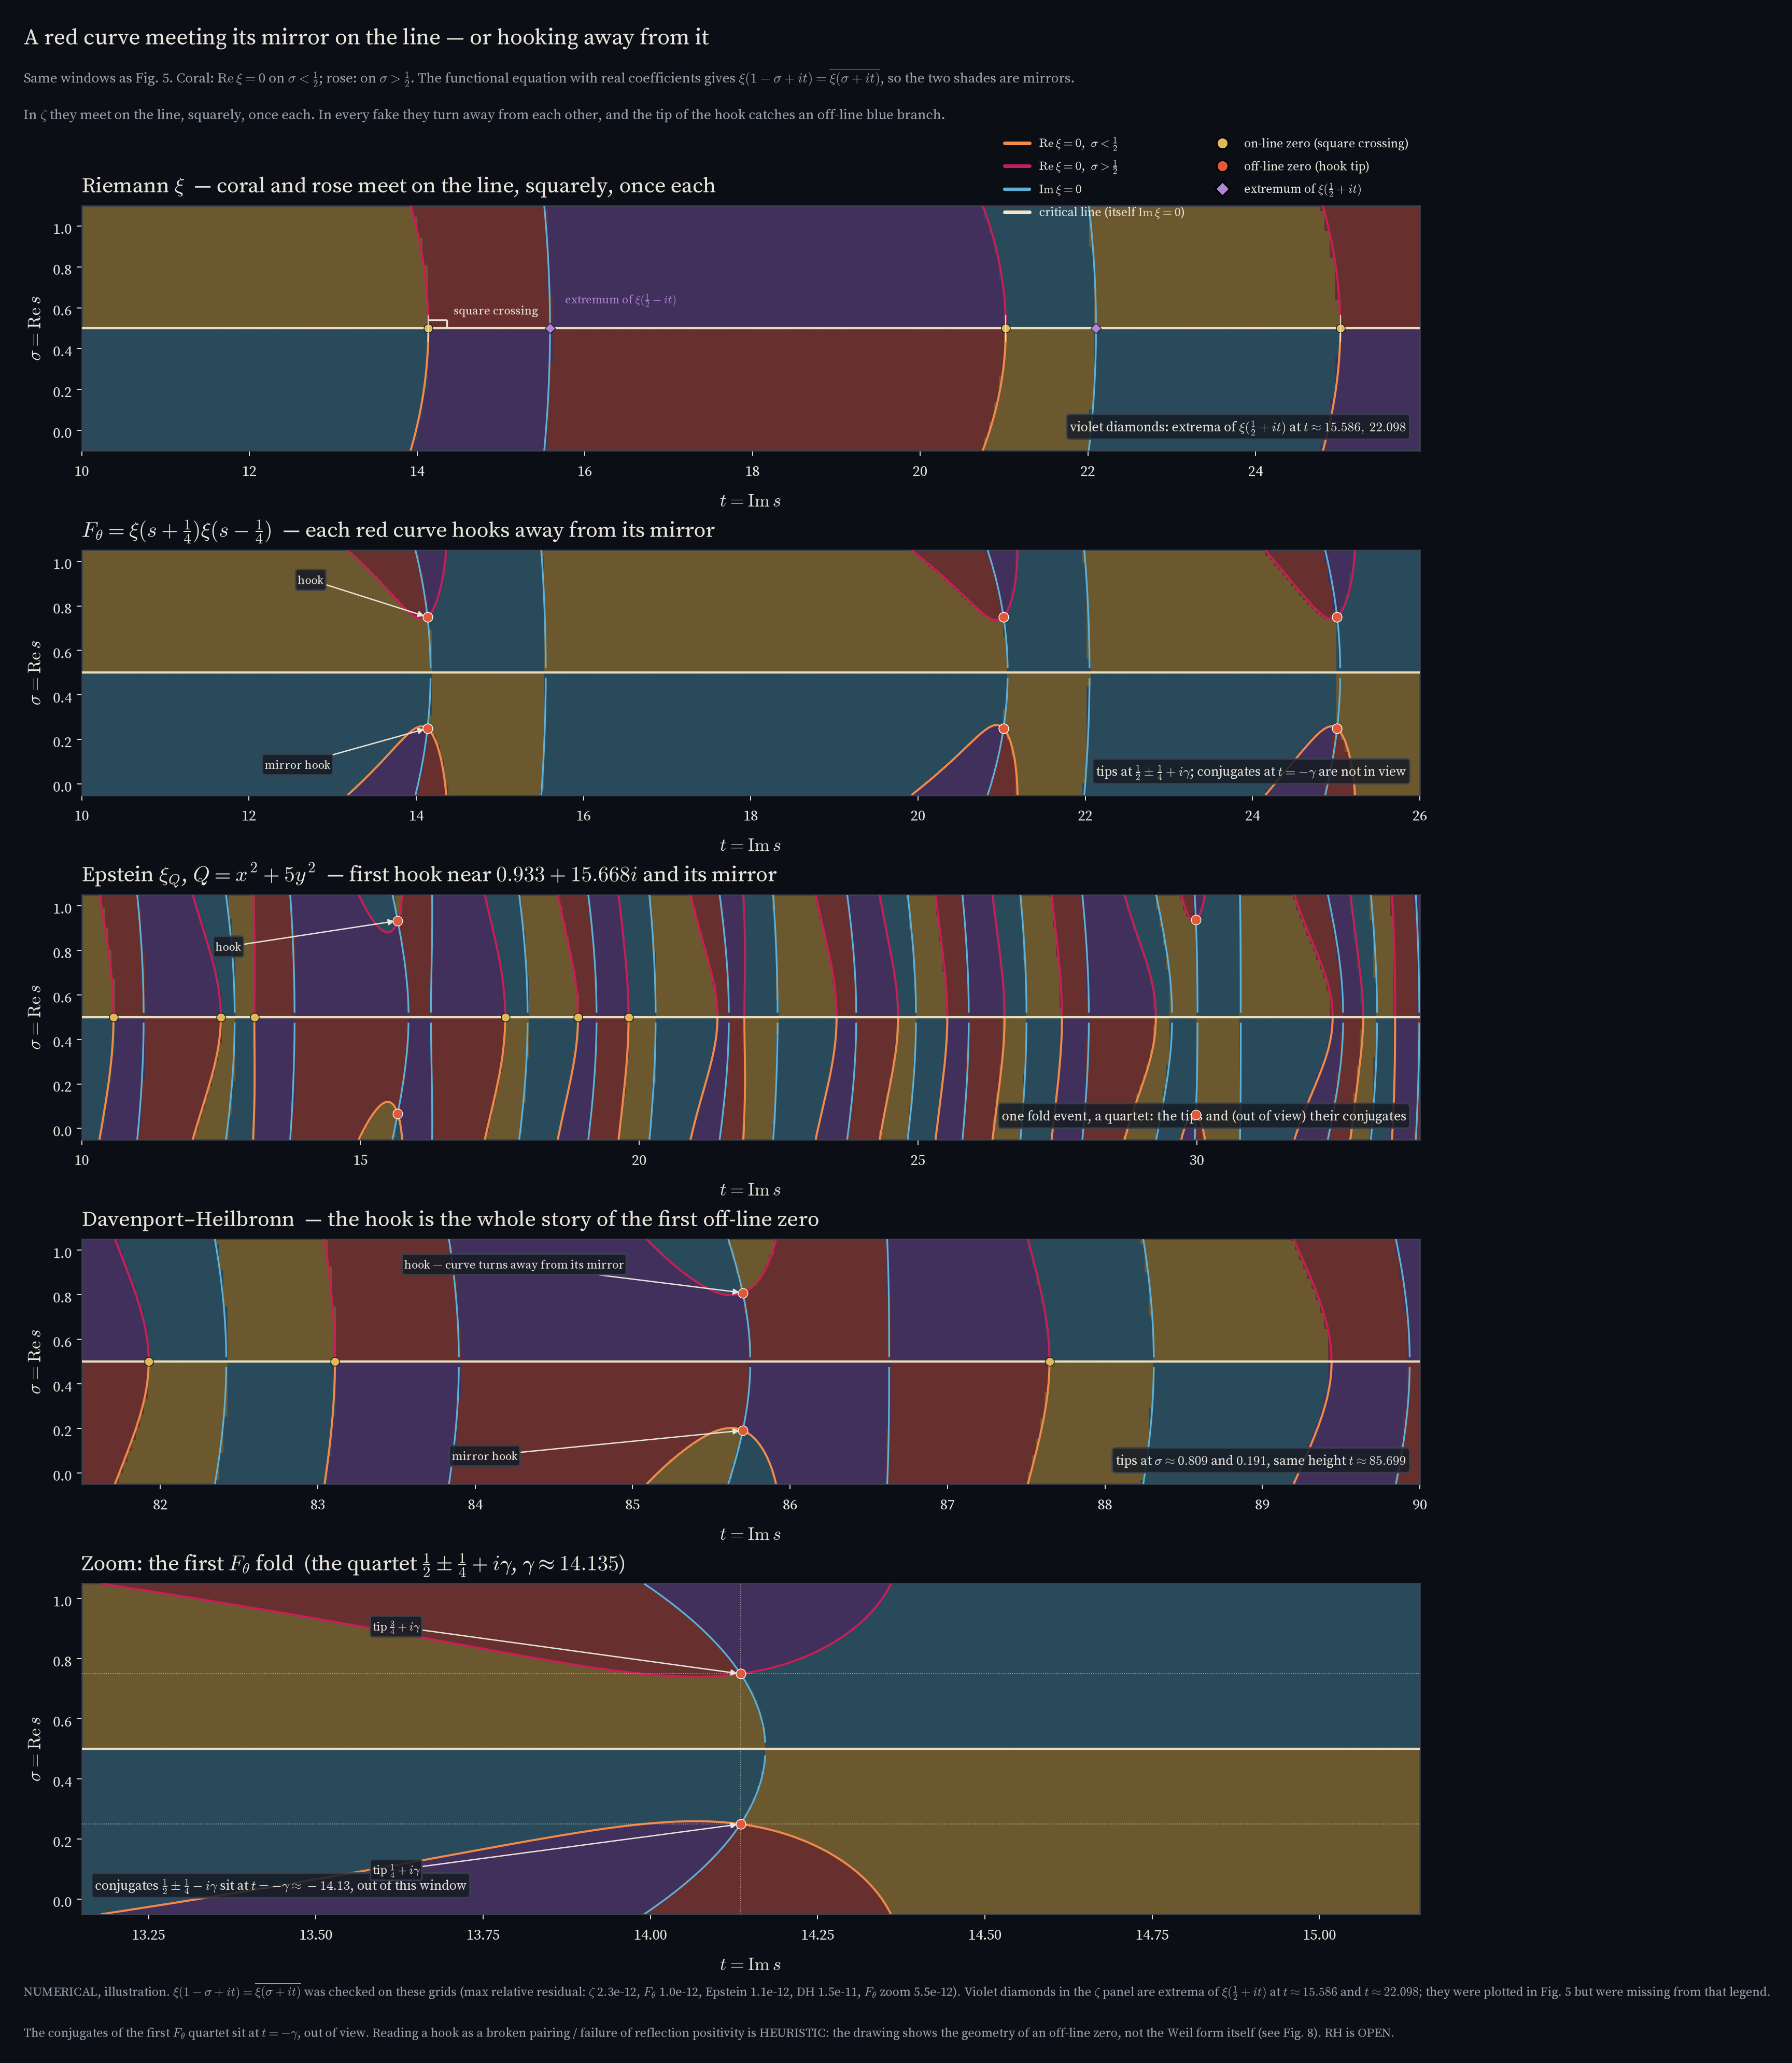
\includegraphics[width=0.9\linewidth]{../round25_viz/fig7_mirror_pairs.png}
\caption{Round 25b (GPPDiscovery5 \texttt{15c6fa8}). Level curves
$\Re\xi=0$ coloured by side of the critical line (the two shades are exact
mirror images under $s\mapsto1-\bar s$), for $\zeta$, $F_{1/4}$, Epstein
($x^2+5y^2$) and Davenport--Heilbronn. For $\zeta$ each curve meets its
mirror squarely on the line. In each control, a curve and its mirror turn
away from each other (a ``hook''), and the tip catches an off-line branch of
$\Im\xi=0$, which is an off-line zero. \NUMERICAL{} illustration; zeros are
plot marks only.}
\label{fig:mirror}
\end{figure}

\begin{itemize}
\item \textbf{Square crossings vs.\ hooks} \NUMERICAL{} (GPPDiscovery5
\texttt{05d6247}, \texttt{15c6fa8}; Fig.~\ref{fig:mirror}). In every window
examined, the curves $\Re\xi=0$ for $\zeta$ cross the critical line once,
squarely, at each simple zero. Every control shows at least one fold
(hook) whose tip is an off-line zero. Zeros off the line are born as a
fold and its mirror, a quartet $\{\rho,\bar\rho,1-\rho,1-\bar\rho\}$. The
viewpoint is the classical ``X-ray'' of $\zeta$ \cite{AriasDeReyna2003} and
the phase portraits of \cite{Wegert2012}.
\item \textbf{The Weil packet test} \NUMERICAL{} (\texttt{15c6fa8}). With
Fej\'er wave packets of width $2\pi/\log X$ centred at height $t$, the Weil
form computed from each model's own explicit formula (arithmetic side only)
stays positive everywhere for $\zeta$ (valley minima $\approx0.005$). At a
control's hook it shows a \emph{peak} with \emph{negative shoulders}, which
sharpen and move toward the hook as $X$ grows. We expect this signature is
largely automatic once a zero is off the line. An off-line zero contributes
a packet term shifted off the real frequency axis, which naturally produces
side lobes. So it is diagnostic, not explanatory \HEUR.
\item \textbf{The reading} \HEUR. Turbo's reading: a square crossing is a
curve meeting its own mirror image as a true pairing, and a hook is the
pairing failing. In the language of this paper, a square crossing is a
$\Theta$-fixed weight (Lemma~\ref{lem:theta}(iii)), i.e.\ a normalizable
state; a hook is a weight pair $\rho\neq1-\bar\rho$ exchanged by $\Theta$,
which no unitary theory can host (Theorem~\ref{thm:main}). The pictures
therefore show (S) holding or failing. They do not show \emph{why} it
holds for $\zeta$.
\end{itemize}

\subsection{The screw function and a finite certificate}

Suzuki's screw function \cite{Suzuki2022},
\[
\Psi(t)=\sum_\gamma\frac{1-\cos\gamma t}{\gamma^2},
\]
has an equivalent closed form built from the primes, the archimedean factor
and the pole alone. RH is equivalent to several positivity statements about
$\Psi$ \cite{Suzuki2022}. In Round 23 (GPPDiscovery5 \texttt{9be7e6a}) the
closed form was evaluated in ball arithmetic: $\Psi(\log X)>0.0214$ for every
real $X\in[2,10^8]$, \PROVED{} (computer-assisted, \texttt{python-flint}
\texttt{arb}, 160 bits; the attribution to Suzuki was added in Round 24).
This is the $\gamma=0$ slice of a positivity statement. It is a statement
about a finite range only. Unconditionally
$\liminf_{t\to\infty}\Psi(t)\le0$, so no uniform margin exists
(GPPDiscovery5 R23, Thm.~6). Physically, $\Psi$ is a positive spectral
density integrated against a box. Its positivity is the positivity of a
norm, which is what (S) would deliver.

\subsection{Lee--Yang, criticality, and where to look}

\HEUR. Three physical facts suggest where the missing Hilbert space might
come from.
\begin{enumerate}[label=(\roman*)]
\item \emph{Lee--Yang.} For ferromagnetic Ising models, positivity of the
couplings forces the partition-function zeros onto a circle
\cite{LeeYang1952}. Newman showed that a Lee--Yang property of a suitable
measure would imply RH, via the de Bruijn--Newman flow \cite{Newman1976}.
The primon gas~\eqref{eq:primon} is free, so the needed ``ferromagnetic''
structure must come from somewhere other than interactions. The best
candidate is the unitarity of the local factors.
\item \emph{Criticality.} The de Bruijn--Newman constant satisfies
$\Lambda\ge0$ \cite{RodgersTao2020}, while RH is equivalent to
$\Lambda\le 0$. If RH is true, $\zeta$ sits \emph{exactly} at the edge:
the slightest backward heat flow creates off-line zeros. A physicist
recognizes a critical system. Critical systems are exactly the ones
described by conformal field theories, which is consistent with the
conformal-weight reading (S).
\item \emph{Reflection positivity.} In Osterwalder--Schrader
reconstruction \cite{OsterwalderSchrader1973}, a Hilbert space with a
self-adjoint Hamiltonian is \emph{built} from Euclidean correlators that are
positive under a reflection. Here the reflection is
$\Theta:x\mapsto1/x$, the vacuum is $T$, and Weil positivity is precisely
the required reflection positivity. Our audit (Section~\ref{sec:free}) shows
that it cannot be checked prime by prime. A genuinely new idea would be a
\emph{global} reason, using the exact coefficient $1$, that the Euclidean
data of the integers are $\Theta$-positive \OPEN.
\end{enumerate}

%=====================================================================
\section{What is not claimed}
\label{sec:notclaimed}

\begin{itemize}
\item \textbf{The Riemann Hypothesis is not proved.} It remains \OPEN.
\item Theorem~\ref{thm:main} is a \emph{conditional} theorem. Its hypothesis
(Postulate~\ref{pip} or~\ref{pipR}) is \emph{equivalent} to RH
(Remark~\ref{rem:tauto}). We do not claim progress toward establishing the
hypothesis beyond identifying the arithmetic that must be used
(Section~\ref{sec:gap}).
\item The 2D$\to$1D reduction of the shadow pairing is a physical
identification \HEUR. The group theory in each dimension is standard
\PROVED, but no theorem here says that the celestial amplitudes of
\cite{ToupinLoops2026} ``contain'' $\zeta$.
\item The Round 25 pictures and the Weil packet test are \NUMERICAL{}
illustrations. The ``hook = broken pairing'' reading is \HEUR.
\item The certificate $\Psi>0.0214$ on $[\log2,\log10^8]$ is a finite-range
statement. It is not, and cannot be extended to, a uniform bound.
\item No zeta zero is used as an input to any proof in this paper.
\item We do not claim that the Hilbert--P\'olya approaches cited are
incorrect or correct beyond what their authors and published comments state.
\end{itemize}

\subsection*{Acknowledgments}
The physical postulates (P1)--(P4), the principle that $s$ is physical, the
shadow-pairing paper \cite{ToupinLoops2026}, and the local-prime-kernel
model are Daniel Toupin's. The mirror-pair reading of the Round 25 figures
is due to Turbo (Golden Physics Project). Numerical and written work in this
round was done in an audited human--AI session.\\[4pt]
--- Daniel Toupin / Golden Physics Project. This seat: Heart of the Cosmos /
Grok (GPPDiscovery5).

%=====================================================================
\appendix
\section{Numerical checks (\texttt{r26\_checks.py})}
All identities below are classical. The script verifies them in
\texttt{mpmath} at 40 digits (output in \texttt{r26\_checks.json}). No zeros
are used.
\begin{center}
\begin{tabular}{lr}
\toprule
identity & max.\ abs.\ error\\
\midrule
$\Gamma(\tfrac12+i\lambda)\Gamma(\tfrac12-i\lambda)=\pi/\cosh\pi\lambda$ & $5\times10^{-41}$\\
$\Gamma(1+i\lambda)\Gamma(1-i\lambda)=\pi\lambda/\sinh\pi\lambda$ & $1\times10^{-41}$\\
$\Im[\Gamma(\Delta)\Gamma(1-\Delta)]$ at $\Delta=0.7+0.5i$ & $0.714$ (nonzero, as Prop.~\ref{prop:cut1d})\\
$T(x)=x^{-1}T(1/x)$ & $2\times10^{-16}$ (float input)\\
Mellin of $\omega$ at $s=3$ vs.\ $\tfrac12\pi^{-3/2}\Gamma(\tfrac32)\zeta(3)$ & $1\times10^{-42}$\\
$\min_{(0,1)}\eta(\sigma)$, $\max_{(0,1)}\zeta(\sigma)$ (99 points) & $0.502>0$, $-0.509<0$\\
Poisson kernel~\eqref{eq:poisson}, $p=3$, $t=1.7$ & $0$\\
$\Im\xi(\tfrac12+it)/|\xi|$, $t\in\{3,10,20.5,33.3\}$ & $8\times10^{-42}$\\
$\xi(1-\bar s)-\overline{\xi(s)}$ at $s=0.8+12.3i$ & $1\times10^{-43}$\\
$\|\Theta_\alpha f\|=\|f\|$, $\alpha=0,1$ & $0$\\
\bottomrule
\end{tabular}
\end{center}

\begin{thebibliography}{99}\small

\bibitem{AriasDeReyna2003} J.~Arias de Reyna, ``X-ray of Riemann zeta-function,''
arXiv:math/0309433 (2003).

\bibitem{Bargmann1947} V.~Bargmann, ``Irreducible unitary representations of the
Lorentz group,'' Ann.\ of Math.\ \textbf{48} (1947) 568--640.

\bibitem{Bellissard2017} J.~V.~Bellissard, ``Comment on `Hamiltonian for the zeros
of the Riemann zeta function','' arXiv:1704.02644 (2017).

\bibitem{BBM2017} C.~M.~Bender, D.~C.~Brody, M.~P.~M\"uller, ``Hamiltonian for the
zeros of the Riemann zeta function,'' Phys.\ Rev.\ Lett.\ \textbf{118} (2017) 130201.

\bibitem{BerryKeating1999} M.~V.~Berry, J.~P.~Keating, ``The Riemann zeros and
eigenvalue asymptotics,'' SIAM Rev.\ \textbf{41} (1999) 236--266.

\bibitem{BerryKeating1999b} M.~V.~Berry, J.~P.~Keating, ``$H=xp$ and the Riemann
zeros,'' in \emph{Supersymmetry and Trace Formulae: Chaos and Disorder},
NATO ASI Ser.\ B \textbf{370}, Springer (1999) 355--367.

\bibitem{Bombieri2000} E.~Bombieri, ``Remarks on Weil's quadratic functional in the
theory of prime numbers, I,'' Rend.\ Mat.\ Acc.\ Lincei (9) \textbf{11} (2000) 183--233.

\bibitem{BostConnes1995} J.-B.~Bost, A.~Connes, ``Hecke algebras, type III factors
and phase transitions with spontaneous symmetry breaking in number theory,''
Selecta Math.\ (N.S.) \textbf{1} (1995) 411--457.

\bibitem{Connes1999} A.~Connes, ``Trace formula in noncommutative geometry and the
zeros of the Riemann zeta function,'' Selecta Math.\ (N.S.) \textbf{5} (1999) 29--106.

\bibitem{DavenportHeilbronn1936} H.~Davenport, H.~Heilbronn, ``On the zeros of
certain Dirichlet series,'' J.\ London Math.\ Soc.\ \textbf{11} (1936) 181--185; 307--312.

\bibitem{Dobrev1977} V.~K.~Dobrev, G.~Mack, V.~B.~Petkova, S.~G.~Petrova,
I.~T.~Todorov, \emph{Harmonic Analysis on the $n$-Dimensional Lorentz Group and
its Application to Conformal Quantum Field Theory}, Lecture Notes in Physics
\textbf{63}, Springer (1977).

\bibitem{Edwards1974} H.~M.~Edwards, \emph{Riemann's Zeta Function}, Academic Press (1974).

\bibitem{Heyl2013} M.~Heyl, A.~Polkovnikov, S.~Kehrein, ``Dynamical quantum phase
transitions in the transverse-field Ising model,'' Phys.\ Rev.\ Lett.\ \textbf{110}
(2013) 135704.

\bibitem{Julia1990} B.~L.~Julia, ``Statistical theory of numbers,'' in
\emph{Number Theory and Physics}, eds.\ J.-M.~Luck, P.~Moussa, M.~Waldschmidt,
Springer Proc.\ Phys.\ \textbf{47} (1990) 276--293.

\bibitem{Knapp1986} A.~W.~Knapp, \emph{Representation Theory of Semisimple Groups:
An Overview Based on Examples}, Princeton Univ.\ Press (1986).

\bibitem{Knauf1999} A.~Knauf, ``Number theory, dynamical systems and statistical
mechanics,'' Rev.\ Math.\ Phys.\ \textbf{11} (1999) 1027--1060.

\bibitem{Lang1975} S.~Lang, \emph{$SL_2(\R)$}, Addison-Wesley (1975); Springer GTM 105 (1985).

\bibitem{LeeYang1952} T.~D.~Lee, C.~N.~Yang, ``Statistical theory of equations of
state and phase transitions. II. Lattice gas and Ising model,'' Phys.\ Rev.\
\textbf{87} (1952) 410--419.

\bibitem{Newman1976} C.~M.~Newman, ``Fourier transforms with only real zeros,''
Proc.\ Amer.\ Math.\ Soc.\ \textbf{61} (1976) 245--251.

\bibitem{OsterwalderSchrader1973} K.~Osterwalder, R.~Schrader, ``Axioms for
Euclidean Green's functions,'' Commun.\ Math.\ Phys.\ \textbf{31} (1973) 83--112.

\bibitem{PasterskiShaoStrominger2017} S.~Pasterski, S.-H.~Shao, A.~Strominger,
``Flat space amplitudes and conformal symmetry of the celestial sphere,''
Phys.\ Rev.\ D \textbf{96} (2017) 065026.

\bibitem{PotterTitchmarsh1935} H.~S.~A.~Potter, E.~C.~Titchmarsh, ``The zeros of
Epstein's zeta-functions,'' Proc.\ London Math.\ Soc.\ (2) \textbf{39} (1935) 372--384.

\bibitem{Riemann1859} B.~Riemann, ``\"Uber die Anzahl der Primzahlen unter einer
gegebenen Gr\"osse,'' Monatsber.\ Berlin.\ Akad.\ (1859) 671--680.

\bibitem{RodgersTao2020} B.~Rodgers, T.~Tao, ``The de Bruijn--Newman constant is
non-negative,'' Forum Math.\ Pi \textbf{8} (2020) e6.

\bibitem{Selberg1992} A.~Selberg, ``Old and new conjectures and results about a
class of Dirichlet series,'' in \emph{Proc.\ Amalfi Conf.\ on Analytic Number
Theory (1989)}, Univ.\ Salerno (1992) 367--385.

\bibitem{SierraTownsend2008} G.~Sierra, P.~K.~Townsend, ``Landau levels and
Riemann zeros,'' Phys.\ Rev.\ Lett.\ \textbf{101} (2008) 110201.

\bibitem{Sierra2019} G.~Sierra, ``The Riemann zeros as spectrum and the Riemann
hypothesis,'' Symmetry \textbf{11} (2019) 494 [arXiv:1601.01797].

\bibitem{Spector1990} D.~Spector, ``Supersymmetry and the M\"obius inversion
function,'' Commun.\ Math.\ Phys.\ \textbf{127} (1990) 239--252.

\bibitem{Suzuki2022} M.~Suzuki, ``Aspects of the screw function corresponding to
the Riemann zeta-function,'' arXiv:2206.03682.

\bibitem{Tate1950} J.~T.~Tate, ``Fourier analysis in number fields and Hecke's
zeta-functions,'' thesis (Princeton, 1950); in \emph{Algebraic Number Theory},
eds.\ J.~W.~S.~Cassels, A.~Fr\"ohlich, Academic Press (1967) 305--347.

\bibitem{Titchmarsh1986} E.~C.~Titchmarsh, \emph{The Theory of the Riemann
Zeta-Function}, 2nd ed., rev.\ D.~R.~Heath-Brown, Oxford Univ.\ Press (1986).

\bibitem{ToupinLoops2026} D.~Toupin, ``Loop amplitudes from unitarity cuts in
celestial Mellin space: a complete derivation for the scalar box,'' Golden
Physics Project, v19 (August 2026).

\bibitem{Weil1952} A.~Weil, ``Sur les `formules explicites' de la th\'eorie des
nombres premiers,'' Comm.\ S\'em.\ Math.\ Univ.\ Lund, tome suppl.\ (1952) 252--265.

\bibitem{Wegert2012} E.~Wegert, \emph{Visual Complex Functions: An Introduction
with Phase Portraits}, Birkh\"auser (2012).

\end{thebibliography}
\end{document}
